\documentclass[12pt,compress]{beamer}
\usepackage{amsmath}
\usepackage{cmbright}
\usepackage{url}
\usepackage{ucs}
\usepackage[utf8x]{inputenc}
\usepackage[ngerman]{babel}
\usepackage{bbm}
\usepackage{ulem}
\usepackage{multicol}
\usepackage{comment}
\usepackage{setspace}
\usepackage{color}
\usepackage{movie15}
\usepackage{hyperref}
\usepackage{bookman}

\usetheme{Boadilla}
\setbeamertemplate{footline}%{infolines theme}

\usecolortheme{lily}
\usefonttheme{serif}
\useinnertheme{circles}
\setbeamercovered{transparent}
\beamertemplatenavigationsymbolsempty

\definecolor{darkgreen}{rgb}{0,0.5,0}

\hypersetup{
    bookmarks=true,
    unicode=true,
    pdftoolbar=true,
    pdfmenubar=true,
    pdffitwindow=false,
    pdfstartview={FitH},
    pdftitle={Klassisches Chaos und Poincaré-Schnitte},
    pdfauthor={Michael Hartmann},
    pdfsubject={Vortrag über klassisches Chaos in hamiltonschen Systemen am Beispiel des Doppelpendels},
    pdfcreator={vim},
    pdfproducer={pdflatex},
    pdfkeywords={Doppelpendel} {Chaos} {Poincare},
    pdfnewwindow=true,
    colorlinks=true,
    linkcolor=black,
    citecolor=green,
    filecolor=magenta,
    urlcolor=darkgreen
}



\title{Klassisches Chaos und Poincaré-Schnitte}
\institute{Kaffeeseminar}
\author{Michael Hartmann}
\date{2. Mai 2013}


\titlegraphic{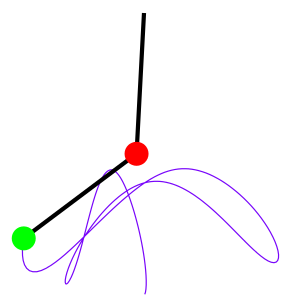
\includegraphics[scale=0.4]{title.png}}


\begin{document}

\begin{frame}
    \titlepage
\end{frame}


\frame{
    \frametitle{Überblick}
    \tableofcontents 
}

\section{Was ist ein Doppelpendel?}

\frame {
    \frametitle{Was ist ein Doppelpendel?}

    \begin{center}
    \includemovie[poster,autoplay,controls=true]{7.5cm}{7.5cm}{pendulum.mp4}
    \end{center}
}

\frame {
    \frametitle{Was ist ein Doppelpendel?}

    \begin{minipage}[b]{0.4\textwidth} 
    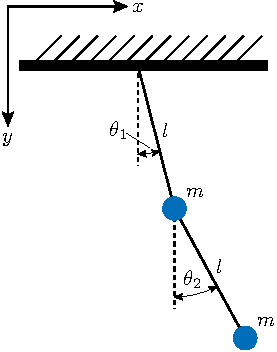
\includegraphics[scale=1]{sketch.pdf}
    \end{minipage}
    \hfill
    \begin{minipage}[b]{0.4\textwidth}
    \begin{align}
    \nonumber
    x_1 &= L_1 \sin\theta_1 \\
    \nonumber
    x_2 &= L_1 \sin\theta_1 + L_2\sin\theta_2 \\
    \nonumber
    y_1 &= -L_1 \cos\theta_1 \\
    \nonumber
    y_2 &= -L_1 \cos\theta_1 - L_2 \cos\theta_2
    \end{align}
    \end{minipage}
}

\section{Bewegungsgleichungen}

\frame {
    \frametitle{Lagrange-Funktion}

    \begin{itemize}
    \item Aufstellen der Bewegungsgleichung mit Lagrange \\ (für $m_1=m_2\equiv m$ und $L_1=L_2\equiv L$)
    \begin{equation}
    \nonumber
    \mathcal{L} = T - V
    \end{equation}
    \item potentielle und kinetische Energie
    \begin{align}
    \nonumber
    T &= \frac{1}{2} mv^2 = \frac{1}{2} m \left(\dot{x}_1^2 + \dot{y}_1^2 + \dot{x}_2^2 + \dot{y}_2^2\right) \\
    \nonumber
    V &= mgL \left(3-2\cos\theta_1-\cos\theta_2\right)
    \end{align}
    \item Lagrange-Funktion
    \begin{align}
    \nonumber
    \mathcal{L} =& mL^2\dot{\theta}_1^2 + \frac{1}{2}mL^2\dot{\theta}_2^2 + mL^2\dot{\theta}_1\dot{\theta}_2\cos{(\theta_1-\theta_2)}  \\
    \nonumber
      &- 3mgL + 2mgL\cos\theta_1 + mgL\cos\theta_2
    \end{align}
    \end{itemize}
}

\frame {
    \frametitle{Hamilton-Funktion und Bewegungsgleichungen}

    \begin{itemize}
    \item Hamiltonfunktion
    \begin{equation}
    \nonumber
    H = \sum_i \dot\theta_i p_i - \mathcal{L}
    \end{equation}
    \item Bewegungsgleichungen
    \begin{align}
    \nonumber
    \dot{\theta}_1 &=  \frac{\partial H}{\partial p_1}  &
    \dot{p}_1 &= -\frac{\partial H}{\partial \theta_1}  \\
    \nonumber
    \dot{\theta}_2 &= \frac{\partial H}{\partial p_2} &
    \dot{p}_2 &= -\frac{\partial H}{\partial \theta_2}
    \end{align}
    \end{itemize}
}

\frame {
    \frametitle{Bewegungsgleichungen}

    \begin{align}
    \nonumber
    \dot{\theta}_1 &= \frac{p_1-p_2\cos\Delta}{L^2m\left[1+\sin^2\Delta\right]} & \dot{\theta}_1 &= \frac{2p_2-p_1\cos\Delta}{L^2m\left[1+\sin^2\Delta\right]}
    \end{align}

    \begin{align}
    \nonumber
    \dot{p_1} &= -2mgL\sin\theta_1 - C &    \dot{p_2} &= -mgL\sin\theta_2  + C
    \end{align}

    \begin{equation}
    \nonumber
    C = \frac{p_1 p_2 \sin\Delta - \left[p_1^2+2p_2^2-2p_1p_2\cos\Delta\right]\sin\Delta\cos\Delta}{L^2 m \left[1+\sin^2\Delta\right]}
    \end{equation}

    \begin{equation}
    \nonumber
    \Delta = \theta_1-\theta_2
    \end{equation}
}

\section{Poincaré-Schnitte}

\frame {
    \frametitle{Poincaré-Schnitte}

    \begin{center}
    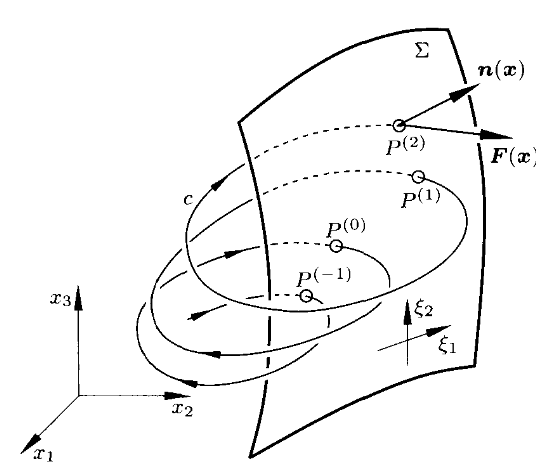
\includegraphics[scale=0.45]{poincare_idea.png}
    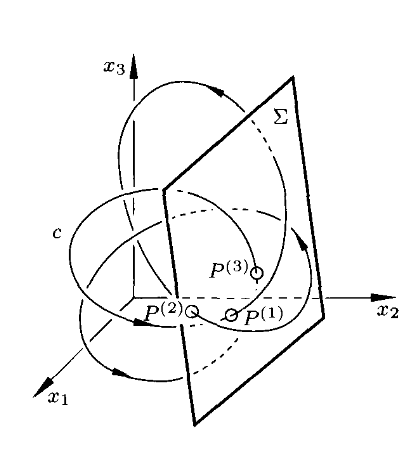
\includegraphics[scale=0.45]{poincare_cycle3.png}
    \end{center}

    \hfill
    \hrule
    \ \\
    {\footnotesize Bildquelle: An Exploration of Chaos, Argyris, Faus, Haase}
}

\frame {
    \frametitle{Vorteile von Poincaré-Schnitten}

    \begin{itemize}
        \item Vergleich verschiedener Anfangsbedingungen
        \item Reduktion der Dimension ohne Verlust an Informationen
        \item qualitatives Verhalten:
        \begin{itemize}
            \item Fixpunkte entsprechen periodische Orbits
            \item Unterscheidung chaotischer und regulärer Bereiche
            \item Linien entsprechen quasiperiodischer Orbits
        \end{itemize}
    \end{itemize}
}

\frame {
    \frametitle{Poincaré-Schnitte für das Doppelpendel}

    \begin{itemize}
        \item abhängig von Parametern: $E$, $L_1$, $L_2$, $m_1$, $m_2$, $g$
        \item 4 Freiheitsgrade: 2 Impulse, 2 Winkel
        \item Energieerhaltung: Trajektorien auf Hyperfläche eingeschränkt
        \item Poincaré-Bedingung $\theta_2 = 0$: noch zwei Variablen
        \item Abbildung von Punkten: $$P(\theta_1^{(0)}, p_1^{(0)}) \mapsto (\theta_1^{(1)}, p_1^{(1)})$$
        \item Durchstoßrichtung beachten!
    \end{itemize}

}

\frame {
    \frametitle{Poincaré-Schnitt für $E=15$}

    \begin{center}
    \includegraphics[width=0.65\textwidth]{E=15.pdf}
    \end{center}
}

\frame {
    \frametitle{Fixpunkte im Poincaré-Schnitt}

    \begin{minipage}[b]{0.3\textwidth} 
    \includegraphics[scale=0.35]{E=15.pdf}
    \end{minipage}
    \hfill
    \begin{minipage}[b]{0.6\textwidth}
    \begin{itemize}
    \item Elliptische Fixpunkte
    \begin{itemize}
    \item Orbit stabil
    \end{itemize}
    \item Hyperbolische Fixpunkte
    \begin{itemize}
    \item Orbit instabil
    \item liegt im chaotischen Bereich
    \item anfällig gegen Störungen
    \end{itemize}
    \item Chaos
    \end{itemize}
    \end{minipage}
}

\frame {
    \frametitle{Orbits}

    \begin{minipage}[b]{0.4\textwidth} 
    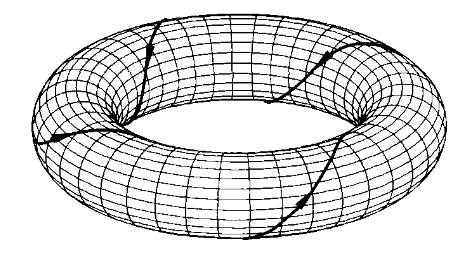
\includegraphics[scale=0.4]{torus_period.png} \\
    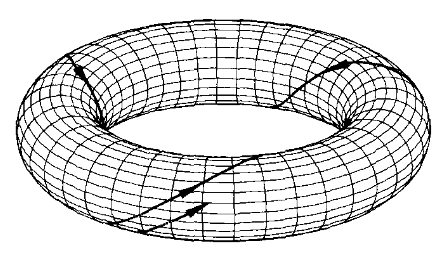
\includegraphics[scale=0.4]{torus_quasi.png}
    \end{minipage}
    \hfill
    \begin{minipage}[b]{0.5\textwidth}
    \begin{itemize}
    \item um elliptische Fixpunkte quasiperiodische Orbits
    \item dazwischen: beliebig viele periodische Orbits
    \end{itemize}
    \begin{center}
    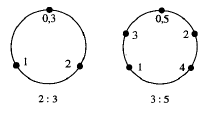
\includegraphics[scale=0.7]{ratio.png}
    \end{center}
    \end{minipage}

    \hfill
    \hfill
    \hrule
    \ \\
    {\footnotesize Bildquelle: An Exploration of Chaos, Argyris, Faus, Haase}
}

\frame {
    \frametitle{Chaos in hamiltonischen Systemen}

    \begin{itemize}
        \item Liouville-Theorem
        \begin{itemize}
        \item Phasenraumvolumen ist inkompressibel
        \item keine Attraktoren
        \end{itemize}

        \item Poincaré-Birkhoff--Theorem
        \item Selbstähnlichkeit
        \item KAM-Theorem
    \end{itemize}

    \vfill
    \hfill
    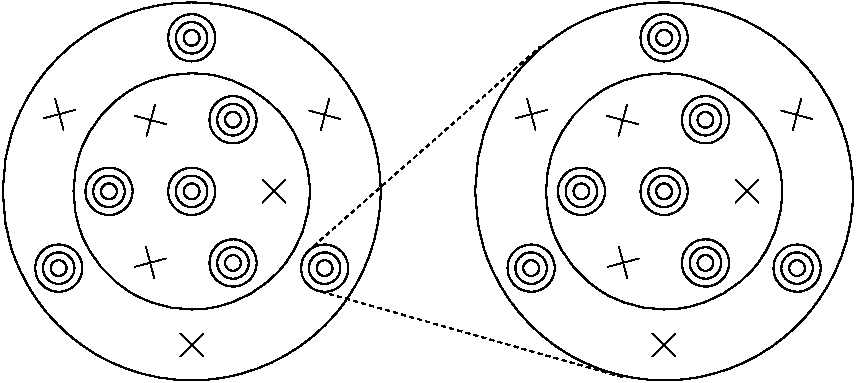
\includegraphics[scale=0.5]{similar.pdf}
}

\section{Beispiele}

\frame {
    \frametitle{Beispiel -- stabiler periodischer Orbit}

    \begin{center}
    \includemovie[poster,autoplay,controls=true]{7.5cm}{7.5cm}{stabil1.mp4}

    $E=15$, $\theta_1=0$, $p_1=2.63362868$
    \end{center}
}

\frame {
    \frametitle{Beispiel -- stabiler periodischer Orbit}

    \begin{center}
    \includemovie[poster,autoplay,controls=true]{7.5cm}{7.5cm}{stabil2.mp4}

    $E=15$, $\theta_1=0$, $p_1=-2.78854801$
    \end{center}
}

\frame {
    \frametitle{Beispiel -- instabiler periodischer Orbit}

    \begin{center}
    \includemovie[poster,autoplay,controls=true]{7.5cm}{7.5cm}{periodisch_instabil.mpeg}

    $E=15$, $\theta_1=0$, $p_1=-4.10536235$
    \end{center}
}

\frame {
    \frametitle{Beispiel -- quasiperiodischer Orbit}

    \begin{center}
    \includemovie[poster,autoplay,controls=true]{7.5cm}{7.5cm}{quasiperiodisch.mp4}

    $E=15$, $\theta_1=0$, $p_1=-5$
    \end{center}
}

\frame {
    \frametitle{Beispiel -- Chaos}

    \begin{center}
    \includemovie[poster,autoplay,controls=true]{11cm}{5.5cm}{chaos.mp4}
    links: $E=15$, $\theta_1=0.8$, $p_1=-4$ \\
    rechts: $E=15$, $\theta_1=0.8$, $p_1=-4.01$
    \end{center}
}

\frame {
    \frametitle{Poincaré-Schnitt in Abhängigkeit von $E$}

    \begin{center}
    \includemovie[poster,autoplay,controls=true]{7.5cm}{7.5cm}{bifurkationen_E.mpeg}
    \end{center}
}


\end{document}
